\documentclass[a4paper,oneside,12pt]{book}

% Variable definitions
\newcommand{\thesistitle}{HubSpot Software Engineering Internship} % Your thesis title, this is used in the title and abstract
\newcommand{\degree}{MAI (Computer Engineering)} % Your degree name, this is used in the title page and abstract
\newcommand{\typeofthesis}{Internship Report} % dissertation, Final Year Project, report, etc.
\newcommand{\authorname}{Stefano Lupo} % Your name, this is used in the title page and PDF stuff
\newcommand{\authorid}{14334933} % Your ID
\newcommand{\keywords}{HubSpot, Software Engineering, Programming, Computer Engineering, 4E4 Internship} % Keywords for your thesis
\newcommand{\school}{\href{http://www.scss.tcd.ie}{School of Computer Science and Statistics}} % title page

\title{\thesistitle}
\author{\authorname}

% Custom commands
\newcommand{\team}{Email Sending Infrastructure}

% Configure output pdf properties
\AtBeginDocument{
\hypersetup{pdftitle=\thesistitle}
\hypersetup{pdfauthor=\authorname}
\hypersetup{pdfkeywords=\keywords}
\hypersetup{pdfsubject=\degree}
}

% Language and font encodings
\usepackage[T1]{fontenc} 
\usepackage[utf8]{inputenc}
\usepackage[english]{babel}

% Bibliographical stuff
\usepackage[round,sort,comma,numbers]{natbib}

% Document size
% include showframe as an option if you want to see the boxes
\usepackage[a4paper,top=2.54cm,bottom=2.54cm,left=2.54cm,right=2.54cm,headheight=16pt]{geometry}
\pagestyle{plain} % Embrace simplicity!

% Useful packages
\usepackage{amsmath}
\usepackage[autostyle=true]{csquotes} % Required to generate language-dependent quotes in the bibliography
\usepackage[pdftex]{graphicx}
\usepackage[colorinlistoftodos]{todonotes}
\usepackage[colorlinks=true, allcolors=black]{hyperref}
\usepackage{caption} % if no caption, no colon
\usepackage{sfmath} %use sans-serif in the maths sections too
\usepackage[parfill]{parskip}    % Begin paragraphs with an empty line rather than an indent
\usepackage{setspace} % to permit one-and-a-half or double spacing
\usepackage{enumerate} % fancy enumerations like (i) (ii) or (a) (b) and suchlike
\usepackage{booktabs} % To thicken table lines
\usepackage{fancyhdr}

%%%%%%%%%%%%%%%%%%%%%%%%%%%%%%%%%%%%%%%%%%%%%%%%%%%%%%%%%%%%%%%%%%%%%%%%
% My Packages
\usepackage{enumitem} %Nested lists a la TOC (plan)
\setlist[enumerate]{label*=\arabic*.}

\usepackage{scrextend}  % List with description all descriptions tabbed as wide as longest
\addtokomafont{labelinglabel}{\sffamily} % Who knows what this does


%%%%%%%%%%%%%%%%%%%%%%%%%%%%%%%%%%%%%%%%%%%%%%%%%%%%%%%%%%%%%%%%%%%%%%%%

% Default to Sans-Serif
\renewcommand{\familydefault}{\sfdefault}

% Options: Sans-Serif, Computer Modern(latex default), palatino
\usepackage{mathpazo} % math fonts
\usepackage{palatino} % nicer font

% Use continuous equation numbers
\renewcommand{\theequation}{\arabic{equation}} 

% Format Chapter headings appropriately
\usepackage{titlesec}
\titleformat{\chapter}[hang] 
{\normalfont\huge\bfseries}{\thechapter}{1cm}{} 

\frontmatter
\begin{document}
\begin{titlepage}

\center % Center everything on the page

%% All the text parameters should be taken from the start of the main.tex file.
%% You should only alter stuff here if you want to change the layout

%----------------------------------------------------------------------------------------
%	LOGO SECTION
%----------------------------------------------------------------------------------------
%% Choose one of the following -- a colour or black-and-white logo


\includegraphics{title/Trinity_RGB_transparent_main.png}\\[1cm] 
%
\includegraphics[width=12cm]{title/black-stacked-trinity.jpg}\\[1cm] 

\Large \school\\[1.5cm] % Minor heading such as course title
\ifdefined\department
\large \department\\[1.5cm] % Minor heading such as course title
\fi

%----------------------------------------------------------------------------------------
%	TITLE SECTION
%----------------------------------------------------------------------------------------
\makeatletter
{ \huge \bfseries \thesistitle}\\[1.5cm] % Title of your document
 

%----------------------------------------------------------------------------------------
%	AUTHOR SECTION
%----------------------------------------------------------------------------------------

\ifdefined\authorid
\authorname\\ % Your name
\authorid\\[2cm] % Your Student ID
\else
\authorname\\[2cm] % Your name
\fi

%----------------------------------------------------------------------------------------
%	DATE SECTION
%----------------------------------------------------------------------------------------

{\large \today}\\[2cm] % Date, change the \today to a set date if you want to be precise

 
%----------------------------------------------------------------------------------------
%	TYPE OF THESIS SECTION
%----------------------------------------------------------------------------------------
 A \typeofthesis\ submitted in partial fulfilment\\of the requirements for the degree of\\
\degree

\vfill % Fill the rest of the page with whitespace

\end{titlepage}
\pagenumbering{roman}


\mainmatter
\section*{\Huge{Declaration}}
\vspace{1cm}
I hereby declare that this project is entirely my own work and that it has not been submitted as an exercise for a degree at this or any other university.

\vspace{1cm}
I have read and I understand the plagiarism provisions in the General Regulations of the University Calendar for the current year, found at \url{http://www.tcd.ie/calendar}.
\vspace{1cm}

I have also completed the Online Tutorial on avoiding plagiarism `Ready Steady Write', located at
\url{http://tcd-ie.libguides.com/plagiarism/ready-steady-write}.
\vspace{3cm}

Signed:~\rule{5cm}{0.3pt}\hfill Date:~\rule{5cm}{0.3pt}

\chapter*{Abstract}
A short summary of the problem investigated, the approach taken and the key findings. This should be around 400 words, or less.

This should be on a separate page.

DESCRIBE THE FOLLOWING LEARNING OUTCOMES (throughout the report, not the abstract)
\begin{enumerate}
	\item contribute to the design and development of systems at forefront of CS research and evaluate their performance
	\item apply theoretical knowledge to solve real world problems
	\item practice and further devel skills in comms, mgmt and teamwork
	\item practice and further develop skills in time management and reporting
	\item contribute to an ethical and profesional work culture
\end{enumerate}

\begin{enumerate}
	\item 
\end{enumerate}

\newpage
\onehalfspacing\raggedright %\raggedright turns off justification and hypenation

\section*{\Huge{Acknowledgements}}
Thanks Mum!

You should acknowledge any help that you have received (for example from technical staff), or input provided by, for example, a company.

\tableofcontents
\listoffigures
\listoftables
\newpage


\section*{\Huge{Nomenclature}}
\begin{tabular}{lp{9cm}l}
A&Area of the wing&$m^{2}$\\
B\\
C& Roman letters first, with capitals\ldots\\
a&then lower case.\\
b\\
c\\
$\Gamma$&Followed by Greek capitals\ldots\\
$\alpha$&then lower case greek symbols.\\
$\beta$\\
$\epsilon$\\
TLA&Finally, three letter acronyms and other abbreviations arranged alphabetically\\
\end{tabular}
\vspace{2cm}

If a parameter has a typical unit that is used throughout your report, then it should be included here on the right hand side.

If you have a very mathematical report, then you may wish to divide the nomenclature list into functions and variables, and then sub- and super-scripts.

Note that Roman mathematical symbols are typically in a serif font in italics.


\begin{enumerate}
	\item Introduction (5 Pages)
	\begin{enumerate}
    	\item Who are HubSpot - 2
        \item The Email Sending Infrastructure Team - 2
        \item Goals of the team or something - 1
    \end{enumerate}
    
    \item Technologies Used (~26 pages, probably excessive)
    \begin{enumerate}
    	\item Java 8 Features (streams, CF, lambdas, Executors) - 5
        \item Kafka - 5
        \item Hadoop - 3
        \item DNS - 3
        \item SMTP - 2
        \item MySql (InnoDB) - 3
        \item HBase (Sync, Idempot, Locks) - 3
        \item ZooKeeper (+ Circus) - 2
        \item RateLimiters, Distributed RateLimiters
    \end{enumerate}
    
    \item HubSpot Methodology (10 Pages)
    \begin{enumerate}
    	\item Java MicroServices - 5
        \item React Native / Redux front end - 4
    \end{enumerate}
    
    \item Major Projects Undertaken (20)
    \begin{enumerate}
    	\item Rebuilt DNS management - 5
        \item Auto DNS for dedicated accounts - 5
    	\item EmailMtaSending Kafka stuff - 5
    \end{enumerate}
    
\end{enumerate}

\chapter{Team Process}
As with any type of team, it is critical that the team is managed appropriately.  

\section{Task Managemenet}
In order to maximize productivity and maintain a healthy workload, a system must be put in place which dictates how team members are assigned units of work. The method used by the \team{} team, was to split tasks up into the following five stages:

\begin{labeling}{In-Progress}
	\item [Backlog] This contains tasks which are of low priority and can be deferred until a later date
	\item [Design] This contains tasks which require a considerable amount of planning before being undertaken. Tasks in this stage often result in discussions amongst the team about how best to tackle the task.
	\item [Ready] Tasks which are sufficiently specified that they can be undertaken. More complex tasks that were once in the design category land here once all of the corresponding details have been decided upon. These are tasks which engineers on the team should choose as a next task upon completion of a task.
	\item [In-Progress] This contains tasks which are currently being worked on (usually) by a single engineer.
	\item [Completed] Tasks which have been completed this week.
\end{labeling}

All of the tasks are managed through an online platform called Waffle\cite{waffle} which presents a \textit{"Waffle Board"} which displays the tasks in each of the above stages. The team concludes each week with a meeting in which the board is inspected and tasks are moved to new stages as appropriate. This provides a great mechanism for monitoring the team's productivity and ensuring that the team is focused on the most important tasks. 
\chapter{Tasks Undertaken}


Throughout the course of the internship, a variety these tasks were undertaken and completed.  

For the sake of brevity a small subset of the most interesting of these tasks are outlined below. 
\chapter{Figures, Tables and Referencing}

\section{Figures}
Graphs, pictures and other images should be included in your report as a numbered, captioned figure. An example is given in Figure \ref{veldis}.

%%%%%%%%%%%%%%%%%%%%%%%%%%%%%%%%%%%%%%%%
\begin{figure}[h]
      \centering
      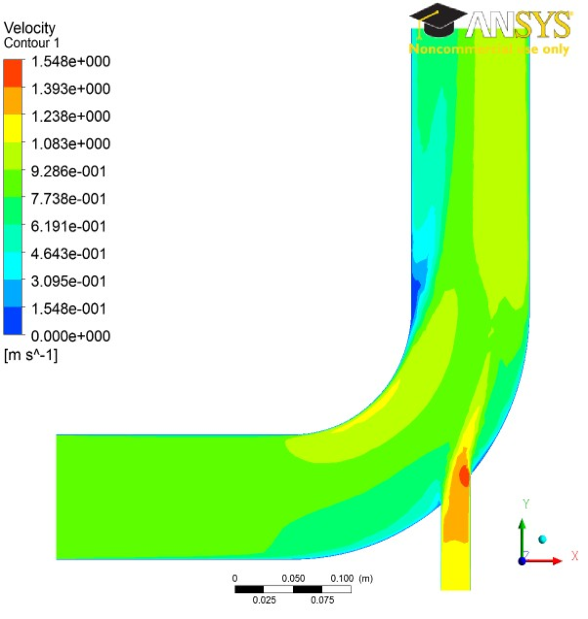
\includegraphics{background/5e1-1.pdf}
      \caption{Velocity distribution on the mid-plane for an inlet velocity for case 1.}
      \label{veldis}
\end{figure}
%%%%%%%%%%%%%%%%%%%%%%%%%%%%%%%%%%%%%%%%

The figure and caption should be centred. The figure numbering starts at 1 at the beginning of each chapter. The caption should provide a brief description of what is being shown. The figure should appear in the document after it is referred to in the text. No figure should be included which is not referred to in the text. Ensure that the size and resolution of images imported from software are sufficient to read any text.

\section{Tables}
Tables are an important way of displaying your results; Table \ref{tab:treatments} is a sample table, adapted from the Master/Doctoral Thesis template at \url{http://www.latextemplates.com/cat/theses}, which was generated with this code:

{\footnotesize
\begin{verbatim}
\begin{table}[b]
\caption{The effects of treatments X and Y on the four groups studied.}
\label{tab:treatments}
\centering
\begin{tabular}{l l l}
\toprule
\textbf{Groups} & \textbf{Treatment X} & \textbf{Treatment Y} \\\midrule
1 & 0.2 & 0.8\\
2 & 0.17 & 0.7\\
3 & 0.24 & 0.75\\
4 & 0.68 & 0.3\\
\bottomrule\\
\end{tabular}
\end{table}
\end{verbatim}
}

\begin{table}[b]
\caption{The effects of treatments X and Y on the four groups studied.}
\label{tab:treatments}
\centering
\begin{tabular}{l l l}
\toprule
\textbf{Groups} & \textbf{Treatment X} & \textbf{Treatment Y} \\
\midrule
1 & 0.2 & 0.8\\
2 & 0.17 & 0.7\\
3 & 0.24 & 0.75\\
4 & 0.68 & 0.3\\
\bottomrule\\
\end{tabular}
\end{table}

Tables are numbered in the same way as figures. Typically tables also have a short caption, but this is not universally true. The number and caption appear above the table, not below as with figures. Again, no table should appear in the report which has not been referred to in the text. Tables should come after they are discussed in the text. The exact formatting of the table depends somewhat on the content of the table, but in general, the text in the table should be the same font and size as the main text. 

\section{Equations}
All equations should be numbered sequentially. Do not restart the numbering at the beginning of each chapter. Unlike figures and tables, you may not need to refer to every equation in the text. You should take care to format equations properly. Do no simply try to use plain text. Use the equation layout facilities. An example of how equations should appear is shown in Equation \ref{sampleequation}. Here is the code for it:

{\footnotesize
\begin{verbatim}
\begin{equation}
\textrm{div}(\underline{u}) = \frac{\delta u}{\delta x} + \frac{\delta v}{\delta y} +
        \frac{\delta w}{\delta z} = 0
\label{sampleequation}
\end{equation} 
\end{verbatim}
}

\begin{equation}
\textrm{div}(\underline{u}) = \frac{\delta u}{\delta x} + \frac{\delta v}{\delta y} + \frac{\delta w}{\delta z} = 0
\label{sampleequation}
\end{equation} 

\section{Referencing published work}
It is important to give appropriate credit to other people for the work that they have shared through publications. In fact, you must sign a declaration in your report stating that you understand the nature of plagiarism. As well as avoiding plagiarism, citing results or data from the literature can strengthen your argument, provide a favourable comparison for your results, or even demonstrate how superior your work is.

There are many styles to reference published work. For example, the parenthetical style (which is also called the Harvard style) uses the author and date of publication (e.g. ``Smith and Jones, 2001''). There is also the Vancouver (or the citation sequence) style, which is shown in this document. In the Vancouver style, the publications are cited using a bracket number which refers to the list in the References section at the end of the report. The references are listed in order that they are cited in the report. A variant is name sequence style in which the publications are referenced by number, but the list is arranged alphabetically. For example, the text might say: several studies have examined the sound field around tandem cylinders generated by flow\cite{fitzpatrick2003flow,finnegan2010experimental}, while other investigations have focused on the effect of an applied sound field on the flow\cite{hall2003vortex}. Papers from conference proceedings\cite{jordan2001array}, books\cite{paidoussis2010fluid} and technical reports\cite{reyes2007power,iea2011} can be dealt with in the same style.

The Vancouver style has the advantage that it is a little more compact in the text and does not distract from the flow of the sentence if there are a lot of citations. However, it has the disadvantage that it is not immediately clear to the reader what particular work has been referenced.

It actually does not matter which particular referencing style is used as long as three important considerations are observed:
\begin{itemize}
\item the referencing style used throughout the document is consistent;
\item all material used or discussed in the text is properly cited;
\item nothing is included in the reference list that has not been cited.
\end{itemize}

This template has a suitable referencing style already set up -- you should use it and use the built-in BibTeX system to manage your references. See above for examples of how to cite a reference and look in the \texttt{sample.bib} file to see BibTeX references. Remember \href{http://scholar.google.com}{Google Scholar} and other search engines will give you BibTeX references for lots of academic publications. Otherwise, you can easily make up your own based on the examples in that file.

\bibliographystyle{unsrtnat}
\bibliography{bibs/sample}

\appendix
\renewcommand{\thechapter}{A\arabic{chapter}}
\chapter{Appendix}
You may use appendices to include relevant background information, such as calibration certificates, derivations of key equations or presentation of a particular data reduction method. You should not use the appendices to dump large amounts of additional results or data which are not properly discussed. If these results are really relevant, then they should appear in the main body of the report.

\section{Appendix numbering}
Appendices are numbered sequentially, A1, A2, A3\ldots The sections, figures and tables within appendices are numbered in the same way as in the main text. For example, the first figure in Appendix A1 would be Figure A1.1. Equations continue the numbering from the main text.


\end{document}